\documentclass[11pt,a4paper,english,oneside, pdf]{article}
\usepackage[margin=2.5cm]{geometry}
\usepackage[utf8]{inputenc} %Permite introducir directamente acentos: á en lugar de \'a etc.
\usepackage{mathtools}
\usepackage{palatino}
\usepackage{graphicx}
\usepackage{hyperref}
\usepackage{xcolor}

\title{Systematics and uncertainties in BACoN}
\author{Carmen Romo Luque}

\graphicspath{{/Users/romoluque_c/Repositories/BACON_romo/analysis_documentation_run3/images/}}

\begin{document}
	\maketitle
	
	
	This document aims to list all the uncertainties and systematics involved in the BACoN experiment.
	
	\section{Geometrical effects}

	How well the SiPMs and PMT collect light from scintillation events at different positions inside the cylindrical vessel.

	\begin{itemize}
		\item Uncertainty in the exact position of the SiPMs with respect to the source. The SiPMs on each row should be at the same distance but we measured it with a rule with 1 mm precision and the base where the SiPMs are placed has a 2 mm thickness.
		
		\item Bending angle for each SiPM. The angles where performed by hand using a compass of 1 degree precision but the base where the SiPMs are placed has a 2 mm thickness. The bases were angled differently depending on the SiPM row.
		
		\item Shadowing effect of the cables on the channels. We tried to reduce this effect as much as we could.
		
		\item Reflectivity of the vessel walls: are the walls reflective? It should be small, but check numbers.
		
		\item Gamma ray path. The exact path of the gamma rays from the americium source through the liquid argon could vary due to absorption and the different Xe concentrations, leading to differences in light yield depending on where the interaction occurs.
	\end{itemize}
	
	
	\section{Uncertainties associated with the source}
	
	\begin{itemize}
		\item Source activity and source uniformity uncertainties. This can affect the expected event rate.

		\item There is a Kapton tape in front of the source to supress the alpha particles emitted by the source to make the system as similar as the LLAMA setup. Could this tape reduce the number of gammas reaching the liquid argon? If so, it should be minimal.
	\end{itemize}
	
	
	\section{SiPM response uniformity}
	
	\begin{itemize}
		\item \textbf{Uniformity of response across the different SiPMs. Even if they are identical and from the same vendor, small differences in manufacturing or operational conditions might introduce variations in their response. We can correct for this by calibrating the channels to obtain the ADC-to-pe conversion factor and normalizing each channel to pe.}
		
		\item \textbf{Quantum efficiency. Fraction of photons that hit the SiPM and are converted into electrical signals. Needs to be taken from the vendor document.}
		
		\item \textbf{Photodetection efficiency of the SiPMs as a function of the wavelength. This should be provided by the vendor.}
		
		\item Temperature dependence. Do fluctuations in the temperature affect the SiPM signals at low energies? I'd say the effect is negligible. Temperature should be very stable and fluctuations of the order of maximum 1 K could happen.
		
		\item There is one SiPM with a quartz window to block 128 nm light and 1 SiPM with polycarbonate window to block all light below 400 nm. These foild might affect the SiPM calibration and the photodetection efficiency.
	\end{itemize}
	
	
	\section{PMT uncertainties}
	
	\begin{itemize}
		\item Gain and efficiency. Like the SiPMs, the PMT gain and quantum efficiency may introduce uncertainties in light detection.
		
		\item Noise level in the PMTs. Is the noise reduced with temperature for PMTs as well? Dark current should be reduced as well.
	\end{itemize}
	
	\section{Argon and xenon uncertainties}
	
	\begin{itemize}
		\item Argon purity fluctuations over time. Impurities could quench the scintillating photons reducing the proporcionality of the signal to the actual energy deposited. The continuous recirculation through the getter can reduce the number of impurities. There shouldn't be fluctuations in the argon impurities. But we could check this by computing the event rate (although the effect of xenon reduction using the xenon trap is also present so how could we distinguish both?).
		
		\item What's the exact amount of argon gas in the ulage? Are all the SiPMs fully covered in liquid? (They should be). How quickly the xenon will come out from the liquid to the ulage? The recirculation process is: liquid, ulage, cold getter and xenon trap.
		
		\item \textbf{Amount of xenon in the argon. How accurately can we measure the concentration of xenon in the liquid argon mixture? In principle with the new setup this should be easier and more accurate.}
		
		\item What's the efficiency of the xenon trap?
		
		\item \textbf{Triplet/Singlet lifetime values. Were they computed with the xenon that argon always contains, or was it removed?} We think the lifetimes were computed with the xenon and other contaminants. The Munich group wanted to operate with uktra pure argon but they didn't measure the lifetimes.
		
		\item \textbf{Is xenon uniformly distributed throughout the detector?} Stefan Schoenert thinks yes, how do we know?
		
		\item Does the calibration of the sensors vary with xenon concentration? It shouldn't.
		
	\end{itemize}
	
	
	\section{Uncertainties in the electronics}
	
	\begin{itemize}
		\item Dark noise. Noise caused by thermal fluctuations in the electronics and cables. It should be negligible at low temperatures. (See Figure \ref{fig:single_pe_shape}).
		
		\item Baseline noise. Electronic circuits, such as preamplifiers and digitizers, always introduce some level of noise. Baseline can be monitored for each channel and since we perform the baseline subtraction (and the computation of such baseline) for every file of data, this effect should not affect the signal.
		
		\item Pick-up noise. Noise coming from external components of the experiment such as the cold head with its vibrations.
		
		\item Pile-up events. I guess it depends on the source activity. I don't think we have pile-up since we only have the gammas now. But the TUM group removed events where 2 pe peaks were detected.
		
		\item Crosstalk between SiPM channels? I'd say it should be negligible in our system.
		
		\item Trigger efficiency? Doug says that our americium source has around 60 kHz rate, resulting in a 10 kHz gamma rate. Could the rate of alphas be computed with the old data?
		
		\item SiPM and PMT timing. Small variations in the timing response of our channels. I'd assume it's minimal.
	\end{itemize}
	
		\begin{figure}[t]
		\begin{center}
			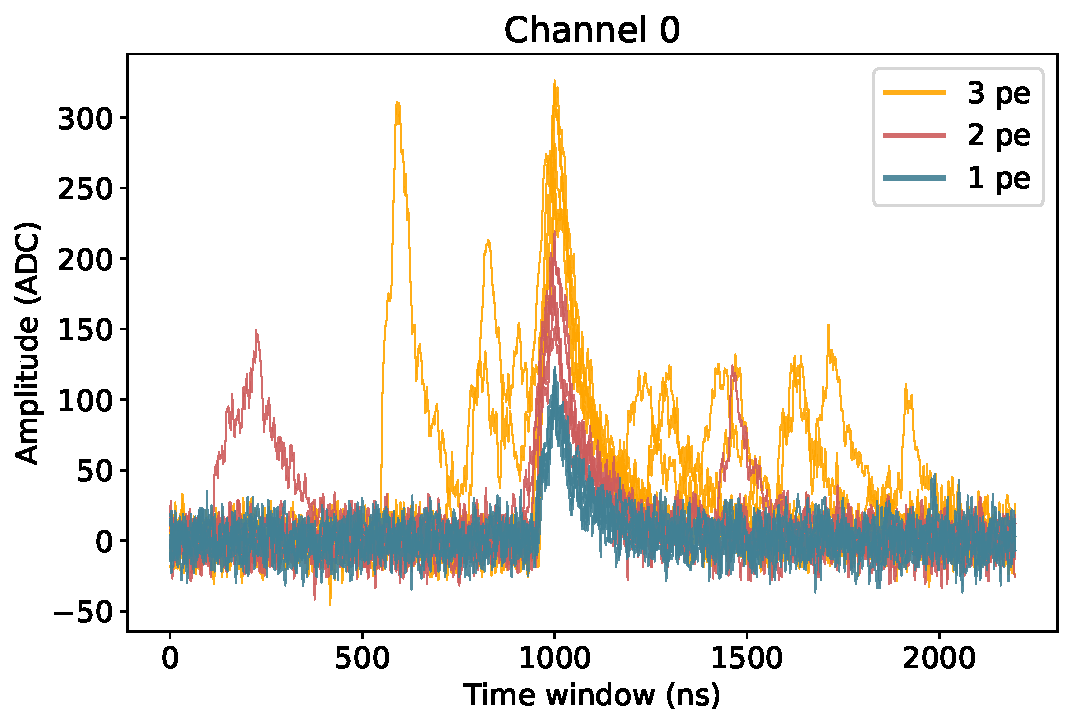
\includegraphics[width=0.8\textwidth]{images/single_pe_shape.pdf}
			\caption{Zoomed waveforms showing the shape of the centered pulses for 1 pe (blue), 2 pe (red) and 3 pe (orange). The dark counts at low temperature are negligible and shouldn't affect the light peaks.}
			\label{fig:single_pe_shape}
		\end{center}
	\end{figure}
	
	
\end{document}